\documentclass{article}%{elsarticle}

\usepackage{lineno,hyperref}
\usepackage{color}
\usepackage{amsfonts}
\usepackage{amsmath}
\usepackage{amssymb}
\usepackage{bm}
\usepackage{mathabx} 
\usepackage{multirow}
\usepackage{subfig}
\usepackage{graphicx}
\usepackage{rotating}
\usepackage{listings}
\usepackage{tikz, pgf}
\usepackage{tikz-3dplot}
\usepackage[linesnumbered, ruled]{algorithm2e}
\def\LW{\dimexpr.25\linewidth-.5em}

\makeatletter
\def\@xfootnote[#1]{%
  \protected@xdef\@thefnmark{#1}%
  \@footnotemark\@footnotetext}
\makeatother

\input macros.tex

\modulolinenumbers[5]

\begin{document}

%%%%%%%%%%%%%%%%%%
%% TITLE 
%%%%%%%%%%%%%%%%%%
\title{A Hybrid Gaussian Process Convolution Neural Network Approach to Single Image Super Resolution}
%% Group authors per affiliation:
\author{Steven I. Reeves \and Dongwook Lee}
%\author[$\dagger$]{Dongwook Lee}%\corref{mycorrespondingauthor}}
%\cortext[mycorrespondingauthor]{Corresponding author}
%\ead{dlee79@ucsc.edu}


\maketitle

\begin{abstract}
Single image super-resolution is a notoriously difficult ill-posed problem. We present a novel hybrid Gaussian Process - Deep
Convolutional Neural Network approach to solving this problem. 
\end{abstract}

%\begin{keyword}
%Gaussian processes; 
%\end{keyword}

%\end{frontmatter}

%\linenumbers


%%%%%%%%%%%%%%%%%%%%%%%%%%%%%%%%%%%%%%%%%%%%%%%%%%
%%%%%% INTRODUCTION %%%%%%%%%%%%%%%%%%%%%%%%%%%%%%%%%%%
%%%%%%%%%%%%%%%%%%%%%%%%%%%%%%%%%%%%%%%%%%%%%%%%%%

\section{Introduction}
\label{sec:introduction}

We propose a new method for upsampling low resolution images from a single base image alone. Single Image Super Resolution (SISR),
is a difficult problem in the field of image processing and computer vision. 

%%%%%%%%%%%%%%%%%%%%%%%%%%%%%%%%%%%%%%%%%%%%%%%%%%
%%%%%% Gaussian Processes %%%%%%%%%%%%%%%%%%%%%%%%
%%%%%%%%%%%%%%%%%%%%%%%%%%%%%%%%%%%%%%%%%%%%%%%%%%
\section{Gaussian Process Modeling}
\label{sec:GP}
The method we are presenting is based on Gaussian Process Modeling, and in this
section we give a brief overview on constructing a Gaussian Process Model. Gaussian Processes
are a family of stochastic processes in which any finite collection of random variables sampled
from this process are joint normally distributed. In a more general sense, Gaussian Processes sample functions
from an infinite dimensional function space. The interpolating routine described in detail in section~\ref{sec:method},
will be drawn from a data-informed distribution space trained on the low resolution data.

To construct a Gaussian Process model, one needs to specify a \textit{prior probability distribution} for
 the function space. Samples (function values evaluated at known locations)
are then used to update this prior probability distribution, and using Bayes' Theorem a \textit{posterior probability
distribution} is generated given the prior and the samples.

\subsection{A statistical introduction to Gaussian Processes}

The construction of the posterior probability distribution over the function space is the heart of
Gaussian Process Modeling. We can draw functions from this data adjusted space to generate an interpolating model.
 Specifically, the posterior may be used to probabilistically predict the value of a function at points where the
function has not been previously sampled.

A Gaussian Process is a collection of random variables, in which any finite collection has a joint Gaussian distribution
\cite{Rasmussen2005}\cite{pattern}.
GPs can be fully defined by two functions:
 a mean function $\bar{f}(\mathbf{x}) = \mathbb{E}[f(\mathbf{x})]$ and a
 covariance function that generates a symmetric, positive-definite kernel
 $K(\mathbf{x}, \mathbf{y}): \mathbb{R}^N\times\mathbb{R}^N \to \mathbb{R}$.

We denote functions $f$ drawn from a GP with mean function $\bar{f}(\mathbf{x})$ and covariance
$K(\mathbf{x}, \mathbf{y})$ as $f\sim \mathcal{GP}(\bar{f}, K)$. Analogous to finite-dimensional
distributions we write the covariance as
\begin{equation} 
K(\mathbf{x}, \mathbf{y}) = \mathbb{E}\left[\left(f(\mathbf{x}) - \bar{f}(\mathbf{x})\right)
\left(f(\mathbf{y}) - \bar{f}(\mathbf{y})\right)\right]
\end{equation}
where $\mathbb{E}$ is with respect to the GP distribution.

One controls the GP by specifying both $\bar{f}(\mathbf{x})$ and $K(\mathbf{x}, \mathbf{y})$,
typically as some hyper-parameterized functions. These hyper-parameters allow us to give the
"character" of functions generated by the posterior (i.e. length scales, differentiability).
Suppose we have a given GP, and $N$ locations $\mathbf{x}_i, i = 1, \dots, N$ at which we collect
samples $f(\mathbf{x}_i$, then we can calculate the likelihood $\mathcal{L}$ -- the probability of
the data given the GP model. Let
$\mathbf{f} = \left[f(\mathbf{x}_1, \dots, f(\mathbf{x}_N) \right]^T $ then the likelihood is
\begin{equation} 
\mathcal{L} \equiv P(\mathbf{f} | \mathcal{GP}(\bar{f}, K)) = (2\pi)^{-N/2} \det |\mathbf{K}|^{-1/2} 
\exp\left[-\frac{1}{2}\left(\mathbf{f} - \bar{\mathbf{f}}\right)\mathbf{K}
\left(\mathbf{f} - \bar{\mathbf{f}}\right)\right]
\label{eq:likely}
\end{equation}
where $\mathbf{K}$  is a matrix generated by
$K_{i,j} = K(\mathbf{x}_i, \mathbf{x}_j)$, $i, j = 1,\dots, N$,
and $\bar{\mathbf{f}} = [\bar{f}(\mathbf{x}_1), \cdots \bar{f}(\mathbf{x}_N)]$. Using these samples we can make a
probabilistic statement about the value of the function $f \sim \mathcal{GP}(\bar{f}, K)$
at a new point $\mathbf{x}_*$. That is, we can model the value of $f(\mathbf{x}_*)$ using this GP model. This
is especially import for Adaptive Mesh Refinement, as we need to construct data at a finer resolution.

An application of Bayes' Theorem along with the conditioning property, directly onto the joint Gaussian prior
given the samples $\mathbf{f}$ give the posterior distribution of the predicted value, $f_*$ given $\mathbf{f}$.
\begin{equation} 
P(f_* | \mathbf{f}) = (2\pi U^2)^{-1/2} \exp\left[- \frac{(f_* - \bar{f}_*)^2}{2U^2}\right].
\end{equation}
Perhaps more important for this application, the posterior PDF gives a new \textit{posterior mean function}
\begin{equation}
\tilde{f}_* \equiv \bar{f}(\mathbf{x}_*) + \mathbf{k}_*^T\mathbf{K}^{-1}\cdot(\mathbf{f} - \bar{\mathbf{f}})
\label{eq:mean}
\end{equation}
and \textit{posterior covariance}
\begin{equation} 
U^2 \equiv k_{**} - \mathbf{k}_*^T\mathbf{K}^{-1}\cdot\mathbf{k}_*.
\end{equation}

\subsection{Choice of Covariance Kernel} 
The choice of covariance kernel can have a dramatic effect on the model 
constructed. Two common kernels that we investigate are the Squared-Exponential 
kernel (see equation~\ref{eq:sqrexp}) and the Mat\'{e}rn kernel(see equation~\ref{eq:matern}).  

The squared exponential kernel essentially assumes that all functions drawn from a Gaussian Process generated with it 
are $C^\infty$ continuous.  
\begin{equation}
K_{sqr}(\mathbf{x}, \mathbf{y}) = \Sigma^2 \exp{\left(-\frac{1}{2l^2}||\mathbf{x} - \mathbf{y}||^2\right)}
\label{eq:sqrexp}
\end{equation}
Equation~\ref{eq:sqrexp} shows that the squared exponential kernel has two hyperparameters, $\Sigma$ and 
$l$. These hyperparameters indicate a prior variance and a length scale respectively. In the Mat\'{e}rn 
family of kernels, we have 3 hyperparameters as indicated in equation~\ref{eq:matern}.

\begin{equation}
K_{mat}(\mathbf{x}, \mathbf{y}) = \Sigma^2 \frac{2^{1-\nu}}{\Gamma(\nu)}\left(\sqrt{2\nu}
\frac{||\mathbf{x} - \mathbf{y}||}{l}\right)^\nu K_{\nu} \left(\sqrt{2\nu}
\frac{||\mathbf{x} - \mathbf{y}||}{l}\right)
\label{eq:matern}
\end{equation}

For the Mat\'{e}rn kernels, $\Sigma$ and $l$ are the same as they are in the squared-exponential. The 
hyperparamter $\nu$ on the other hand, relates the level of "continuousness" of the functions that are 
sampled from a Gaussian Process built with this kernel. The function $K_\nu$ is the modified Bessel 
function of the second kind of order $\nu$. Note that as $\nu$ goes to infinity the Mat\'{e}rn 
covariance kernel converges to the squared-exponential covariance kernel~\cite{Rasmussen2005}.  

Since images are typically processed as whole 0-255 integers, we will use the Mat\'{e}rn kernel to build our model.

\subsection{Why use GP for interpolation?} 
Traditional polynomial based interpolation methods are generally used to interpolation of images. This can be problematic 
in a number of ways. Polynomial based methods are deterministic, and assume the function to be interpolated is continuous.
Often when using a higher order polynomial, the interpolation is more accurate, but is more sensitive to discontinuities 
in the sampled data. 

Gaussian Processes provide a methodology to generate an accurate interpolating model utilizing a patch based 
sampling method that requires less data to be qualitatively similar to bicubic interpolation. 

\begin{figure}
\begin{center}
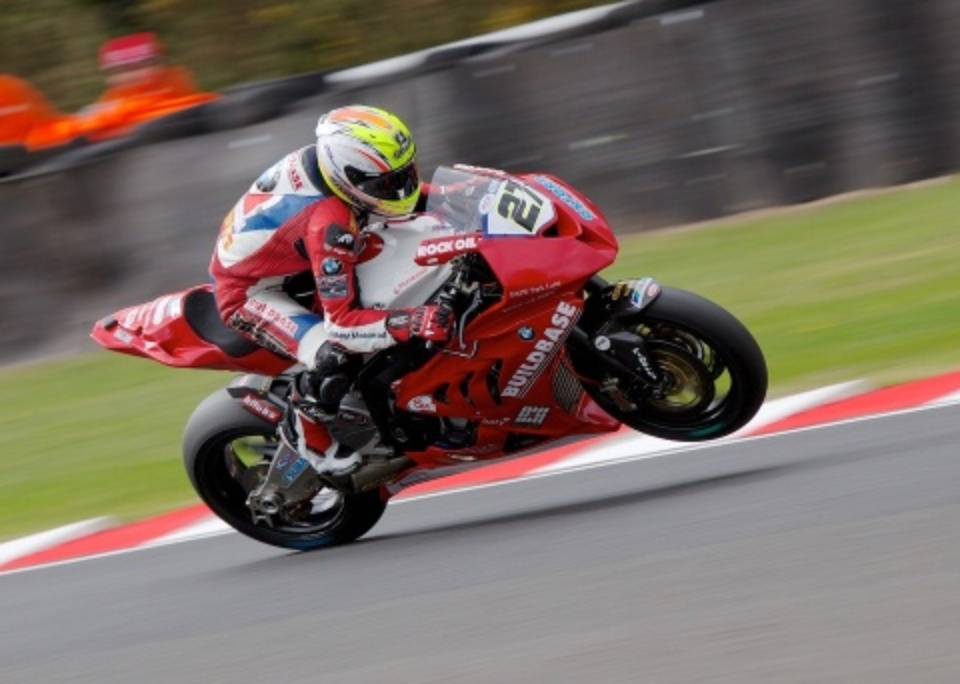
\includegraphics[scale=0.175]{paper_images/interpblin2.jpg}
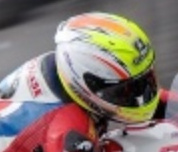
\includegraphics[scale=0.795]{paper_images/interpblin2_zoom.jpg}  
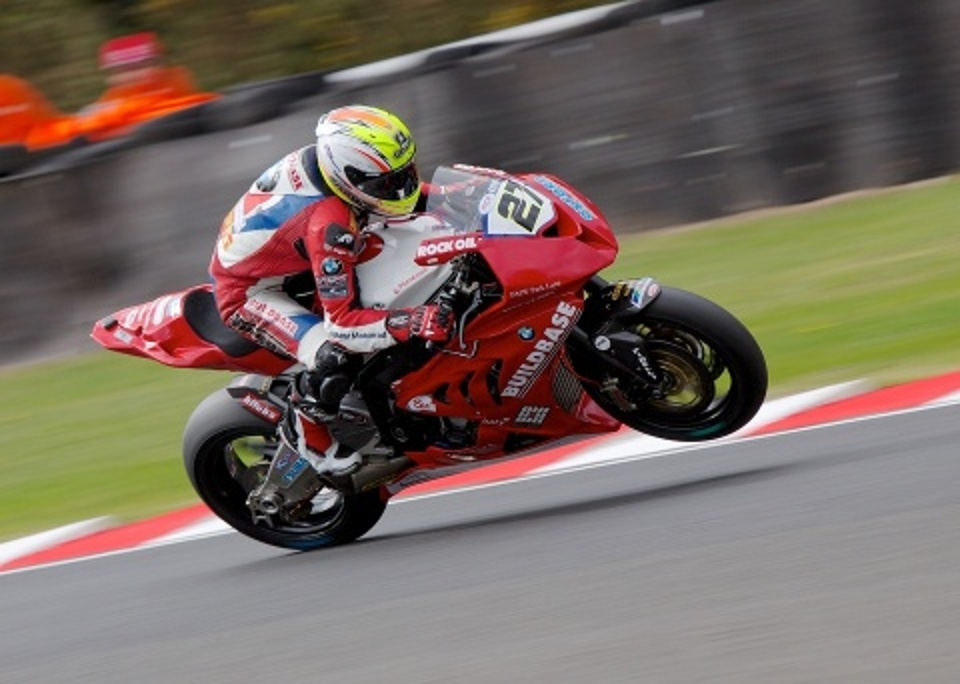
\includegraphics[scale=0.175]{paper_images/interpbic2.jpg}
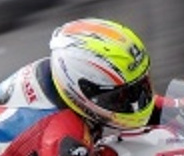
\includegraphics[scale=0.775]{paper_images/interpbic2_zoom.jpg}  
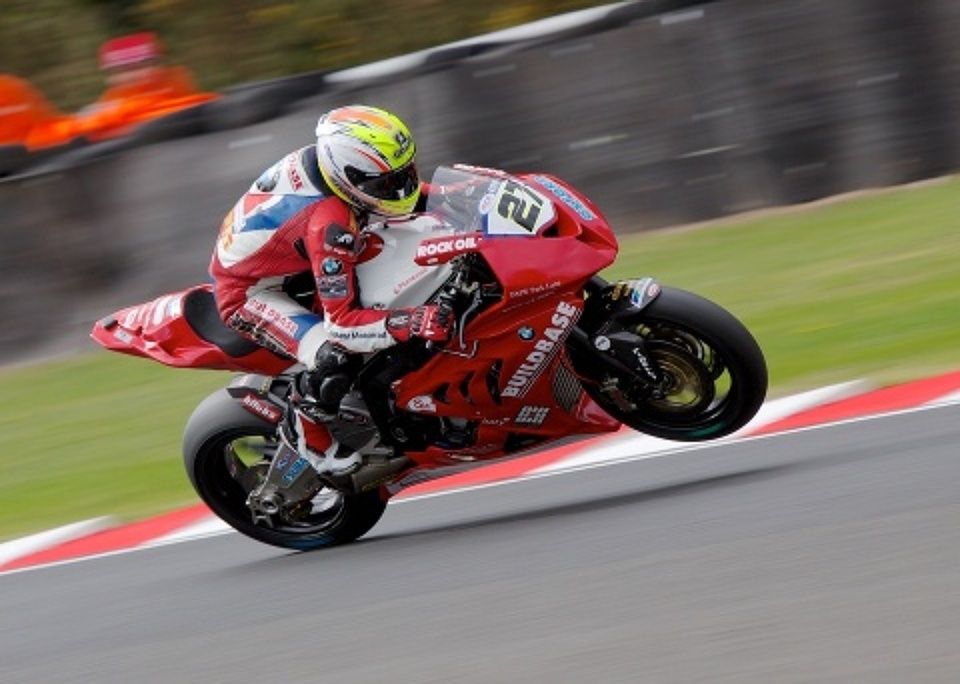
\includegraphics[scale=0.175]{paper_images/sbk_matern32.jpg}
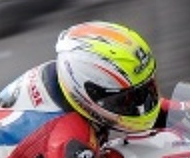
\includegraphics[scale=0.75]{paper_images/sbk_matern32_zoom.jpg}  
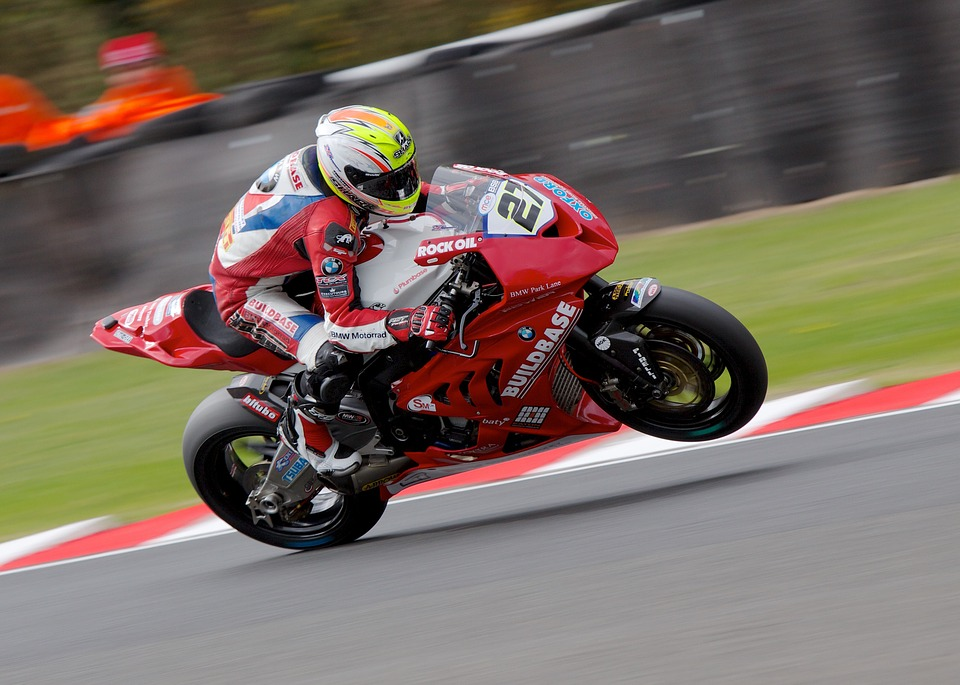
\includegraphics[scale=0.175]{paper_images/superbike_pixabay.jpg}
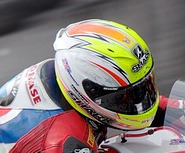
\includegraphics[scale=0.775]{paper_images/truth_zoom.jpg}
\caption{\label{fig:gp} Top-Down, Bilinear Interpolation, Bicubic Interpolation, a Gaussian Process Mat\'{e}rn model and 
the ground truth.}
\end{center} 
\end{figure}

In figure~\ref{fig:gp} we have a photo of a racing motorcyclist that has been downsampled and then interpolated 
using bilinear, bicubic and GP+Mat\'{e}rn $\nu = 3/2$ interpolations and are compared to the ground truth. Notice that the 
result is qualitatively similar between the GP model and the bicubic interpolation. Recall that bicubic interpolation requires
a pixel patch of 4$\times$4 to generate the 16 weights it needs to the interpolation. Our GP model requires a 5 pixel, cross 
shaped stencil, resulting in a matrix multiplication of a $5\times5$ by a 5 element covariance vector to generate weights. 
The bicubic interpolation requires a matrix multiplication of a $16\times 16$ matrix against the data to produce the necessary
weights. Both models then perform dot production between the weight vectors and the stencil data to reviel and interpolated 
point. The matrix for necessary for the bicubic interpolation is known, with a known inverse, whereas the covariance matrix 
for the GP model must be constructed. However, the squared-exponential and Mat\'{e}rn kernels are isotropic that depend on 
distance and not location. Therefore, this matrix can be constructed once for a given set of low resolution images with the 
same pixel count. We will use the property throughout the method we construct.  


\section{Enhancing Convolutional Neural Network} 

Notice that even with higher accurate interpolation schemes, the information 
contained in the lower resolution image does not allow for a complete reconstruction of the higher resolution 
ground truth. We aim bridge the gap between the interpolated image and the ground truth through the use of an 
enhance convolutional neural network (CNN). 

Neural Networks have been employed with good results for many ill posed problems, including single image super resolution
~\cite{IDN}\cite{Enhance}\cite{ISR_DCCN1}\cite{ISR_DCCN2}. 
Many papers involving SISR use end-to-end deep neural networks or use a low 
accuracy interpolation scheme like nearest neighbor. These approaches either 
require the neural network to perform both the interpolation and enhancement, 
or requires a stronger enhancement. 

  


%%%%%%%%%%%%%%%%%%%%%%%%%%%%%%%%%%%%%%%%%%%%%%%%%
%%%%%%% Algorithm %%%%%%%%%%%%%%%%%%%%%%%%%%%%%%%%%%%%%
%%%%%%%%%%%%%%%%%%%%%%%%%%%%%%%%%%%%%%%%%%%%%%%%%%

\section{Hybrid GP-CNN algorithm} 
Our algorithm is an agglomeration of patching, interpolation and enhancing. In order to work on images of any size, we
partition the interpolated image into 128$\times$128 tiles to be enhanced. Then these tiles are stitched together to
form a whole super-resolved image. This technique, allows for the enhancing neural network to utilize fewer weights, to be 
easier trained, and for computational efficiency. 


\begin{algorithm}[H]
lri =  low-resolution image;
 
interp\_i = gp\_interpolate(lri); 

im\_array = partition(interp\_i); 

\For{image in im\_array}{
	enhanced = EnhanceNN(image);
 
	enhance\_array.insert(enhanced); 
} 

high-resolution image = stitch(enhance\_array); 
\caption{SISR Algorithm}  
\end{algorithm}  

%%%%%%%%%%%%%%%%%%%%%%%%%%%%%%%%%%%%%%%%%%%%%%%%%
%%%%%%% References %%%%%%%%%%%%%%%%%%%%%%%%%%%%%%%%%%%%%
%%%%%%%%%%%%%%%%%%%%%%%%%%%%%%%%%%%%%%%%%%%%%%%%%%
\newpage

\section*{}
\label{sec:references}
\bibliographystyle{siam}
\bibliography{mybibfile}




\end{document}
%%% Local Variables:
%%% mode: latex
%%% TeX-master: t
%%% End:
